\section{Projektion laskentamenetelmien vertailu}
\begin{figure}[H]
    \centering
    \captionsetup{width=.9\linewidth}
    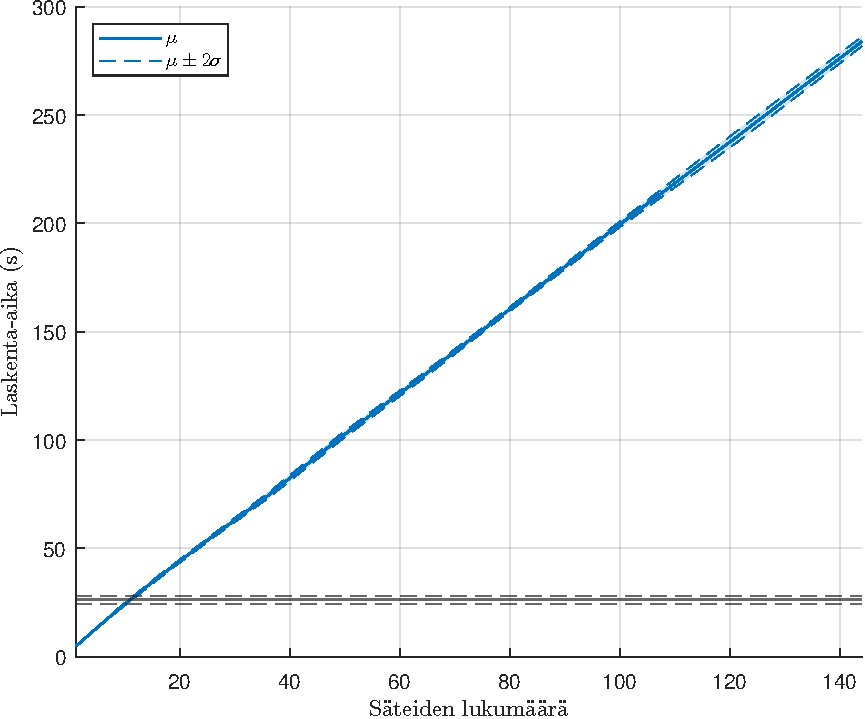
\includegraphics[width=.9\linewidth]{kuvat/laskenta_aika.pdf}
    \caption{Sinisellä viivalla on piirretty mallin 3 keskimääräinen laskenta-aika ($N=100$) säteiden lukumäärän funktiona. Punaisilla katkoviivoilla on havainnollistettu kahden keskihajonnan vaihteluväliä. Rekonstruktiossa kuvan koko oli $128^3$ vokselia sekä algoritmi oli OSEM kahdella iteraatiolla ja 8 osajoukolla. Projektioiden lukumäärä oli 64 ja jokaisessa projektiokuvassa oli $128^2$ pikseliä. Laskennassa käytetty suoritin oli Intel i7-10850H.}
    \label{fig:laskenta_aika}
\end{figure}